\chapter{Depth estimation}


\begin{description}
    \item[Stereo correspondence] \marginnote{Stereo correspondence}
        Given an ideal stereo setup, the depth of each point in the world can be obtained by solving a correspondence problem along rows. Given two points $(u_L, v_L)$ and $(u_R, v_R=v_L)$ in the left and right image, respectively, representing the projection of the same 3D point, its distance $z$ from the camera can be determined using the disparity $d$:
        \[
            \begin{gathered}
                d = u_L - u_R \\
                z = \frac{bf}{d}
            \end{gathered}
        \]
        where $b$ is the baseline (i.e., camera distance) and $f$ is the focal length.

        \begin{figure}[H]
            \centering
            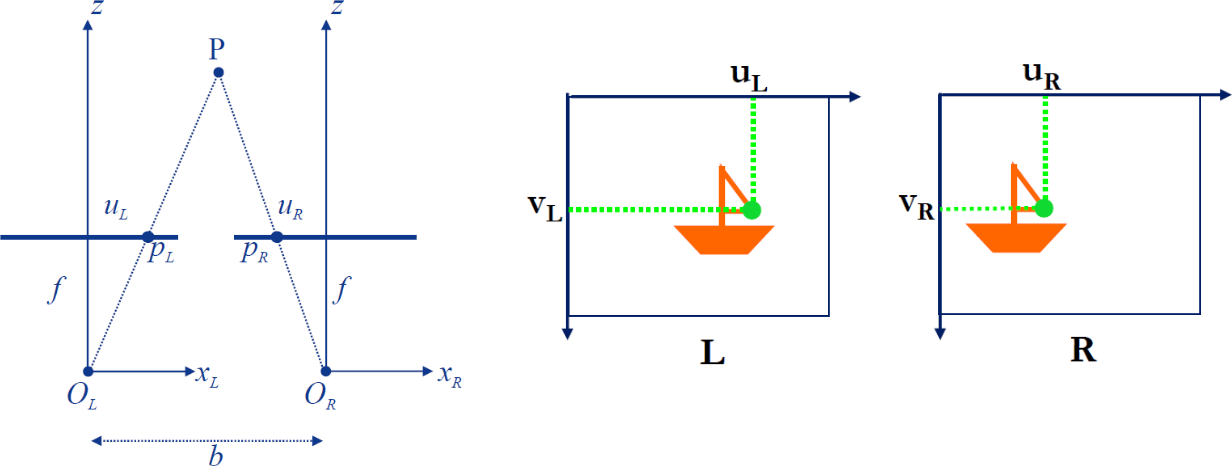
\includegraphics[width=0.65\linewidth]{./img/stereo_correspondence.png}
        \end{figure}
\end{description}

\begin{remark}
    Due to the lack of data, existing models are trained on synthetic data and fine-tuned afterwards on real data.
\end{remark}



\section{Monocular depth estimation}

\begin{description}
    \item[Monocular (single-view) depth estimation] \marginnote{Monocular (single-view) depth estimation}
        Reconstruct the 3D structure of a scene from a single image.

        \begin{remark}
            In principle, this is an ill-posed problem. However, humans are able to solve it through learning.
        \end{remark}
\end{description}


\begin{remark}
    Traditional supervised frameworks (e.g., encoder-decoder) to solve monocular depth estimation have some limitations:
    \begin{itemize}
        \item They require a large amount of realistic synthetic data.
        \item They require expensive hardware for depth measurement when fine-tuning on real data.
    \end{itemize}
\end{remark}


\subsection{Monodepth}

\begin{description}
    \item[Supervised stereo pipeline] \marginnote{Supervised stereo pipeline}
        \phantom{}
        \begin{description}
            \item[Naive approach] 
                A possible solution for depth estimation is to feed a CNN with a pair of synchronized images and make it predict the left (or right) disparity. However, this approach requires to know the ground-truth disparity, which is expensive to obtain.

                \begin{figure}[H]
                    \centering
                    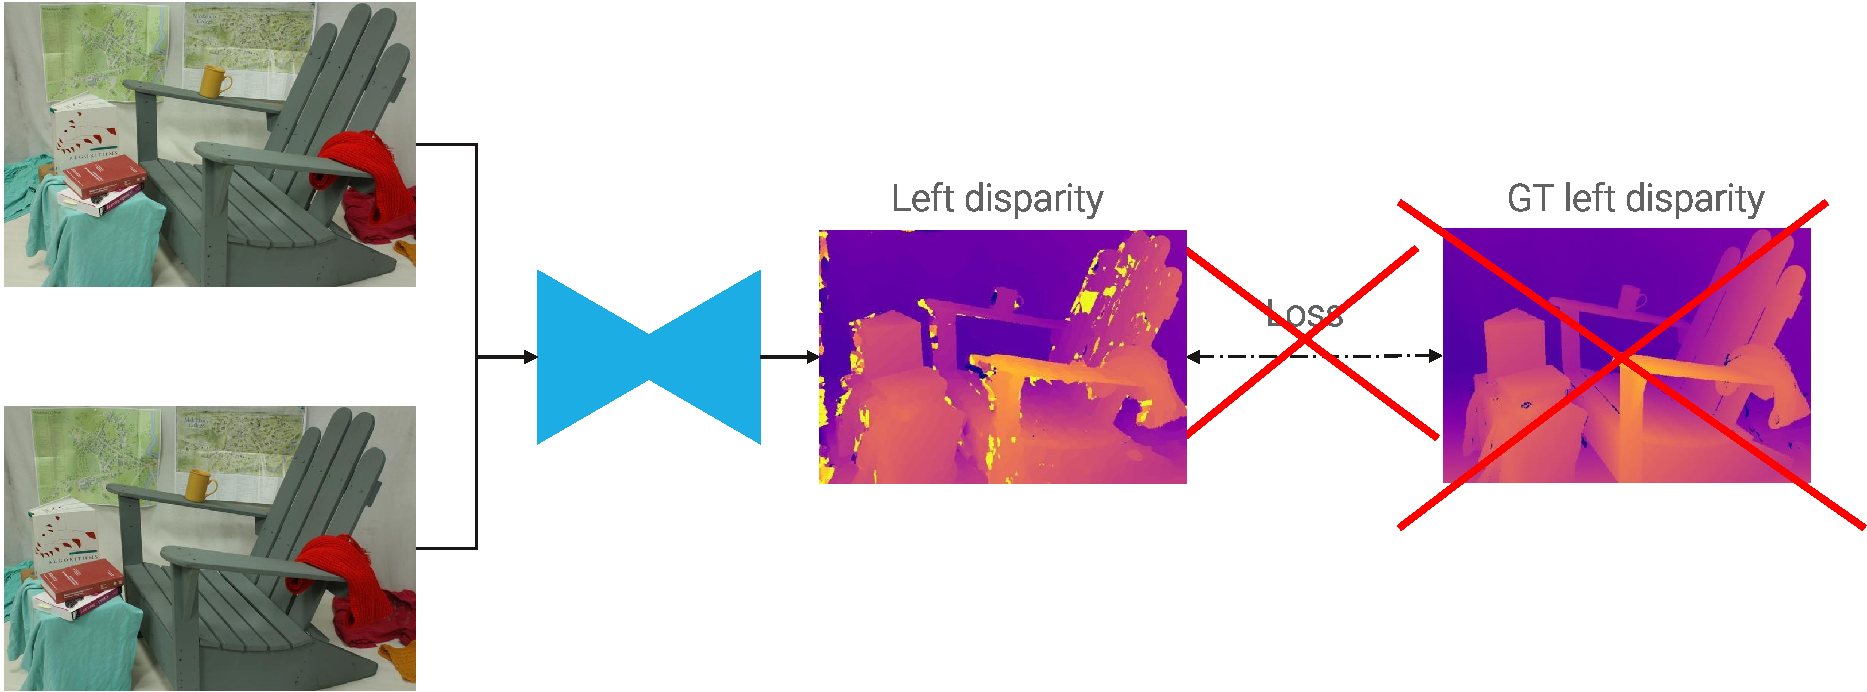
\includegraphics[width=0.7\linewidth]{./img/_stereo_pipeline_naive.pdf}
                \end{figure}

            \item[Reconstruction approach]
                Make the model predict the left disparity which is then used to reconstruct the right image. This works as a pixel $(u, v)$ in the left image with disparity $\tilde{d}$ should appear as the same to the pixel $(u+\tilde{d}, v)$ in the right image.

                \begin{figure}[H]
                    \centering
                    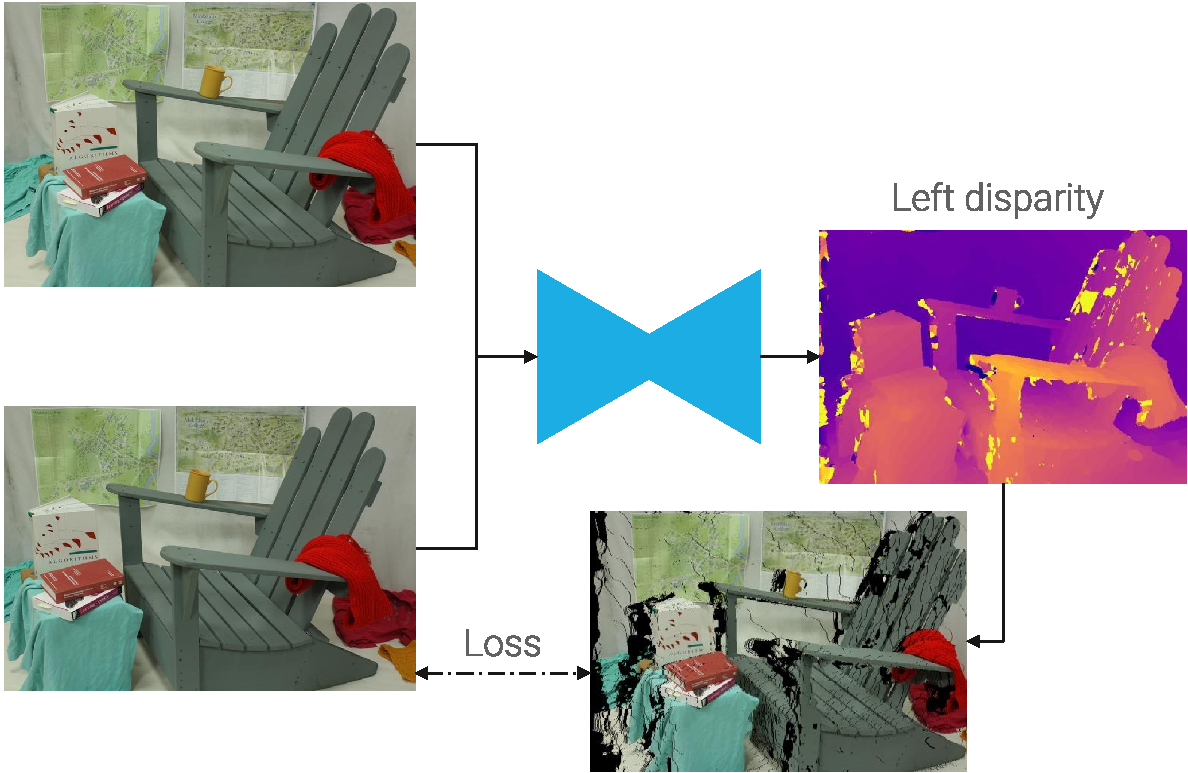
\includegraphics[width=0.45\linewidth]{./img/_stereo_pipeline_reconstruction.pdf}
                \end{figure}
        \end{description}
\end{description}

\begin{description}
    \item[Monodepth]
        Network that takes as input the left (or right) image of a stereo vision system and predicts the left (or right) disparity.

        \begin{description}
            \item[Training (naive)] 
                Once the left disparity has been predicted, it is used to reconstruct the right image.

                \begin{figure}[H]
                    \centering
                    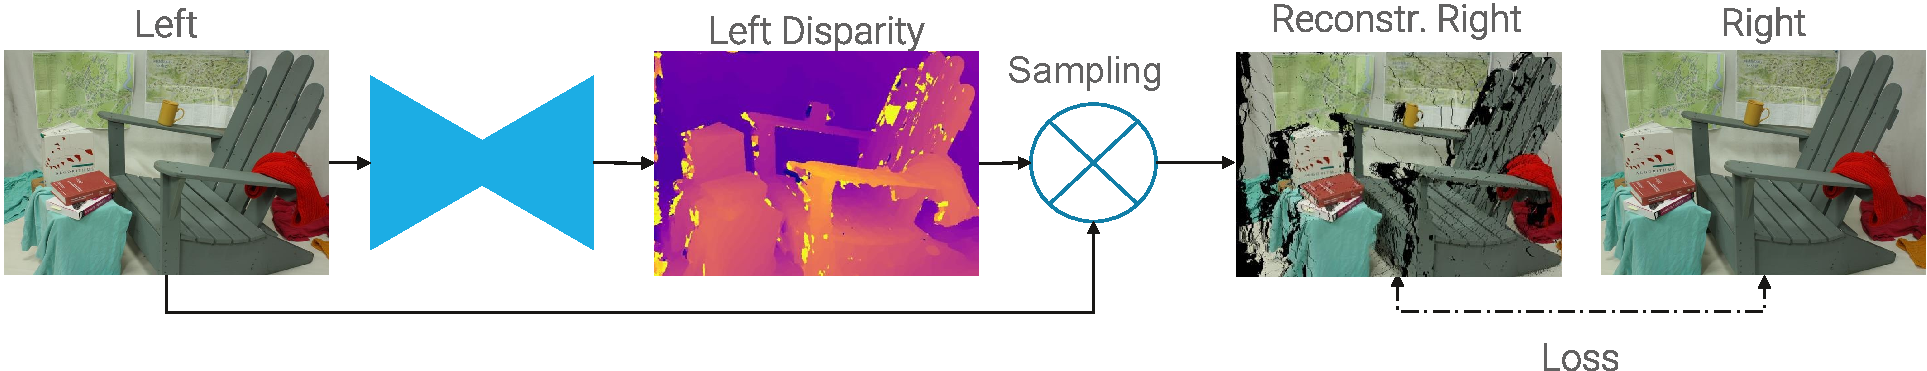
\includegraphics[width=0.8\linewidth]{./img/_monodepth_naive.pdf}
                    \caption{Naive training flow}
                \end{figure}

                \begin{remark}
                    Forward mapping creates holes and is ambiguous as disparities are non-integer values.
                \end{remark}

                \begin{description}
                    \item[(Backward) bilinear sampling] 
                        Compute the right image by determining each pixel of the output backwards and by interpolating it in the left image.

                        \begin{remark}
                            By reconstructing the right image backwards, the estimated disparity will be with respect to the right image, which is not available during inference.
                        \end{remark}

                        \begin{figure}[H]
                            \centering
                            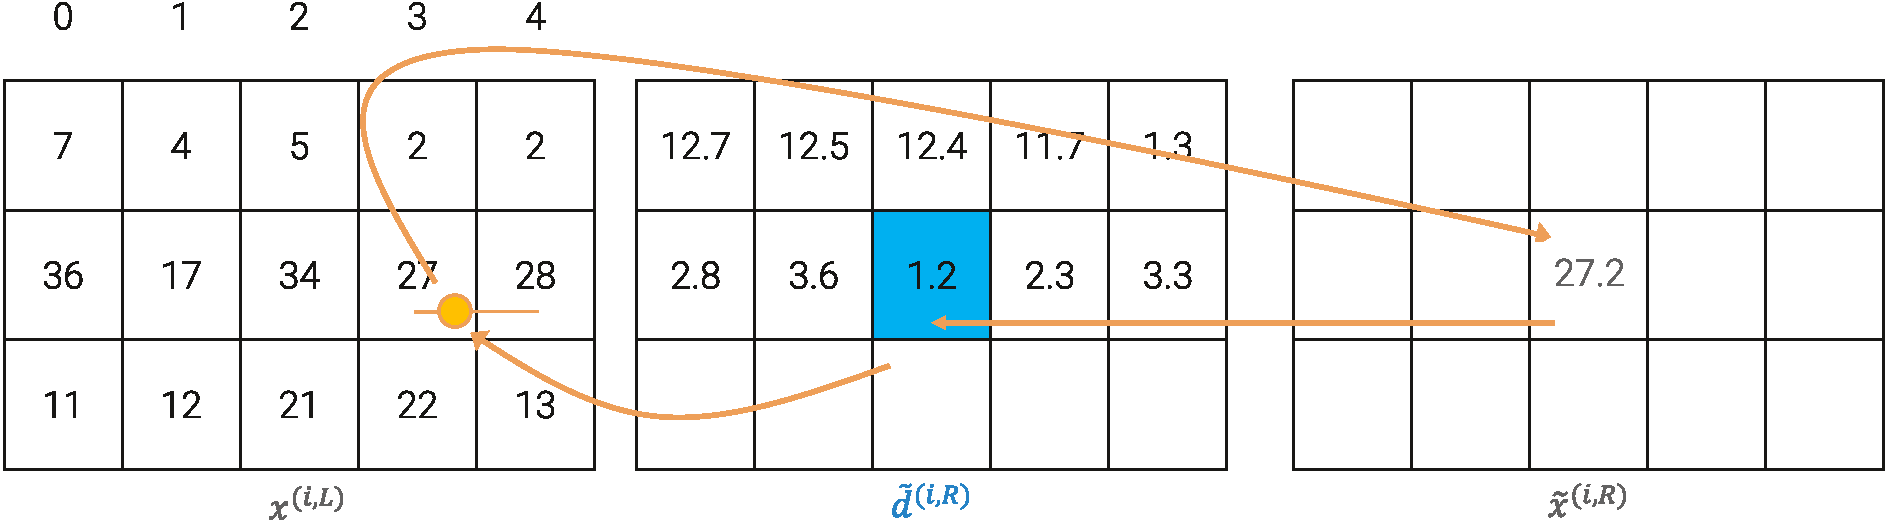
\includegraphics[width=0.65\linewidth]{./img/_monodepth_train_naive.pdf}
                            \caption{Backward reconstruction from the right image}
                        \end{figure}
                \end{description}

            \item[Training (correct)] 
                Once the left disparity has been predicted, it is used to reconstruct the left image by backward mapping from the right image (which is available at train time).

                \begin{figure}[H]
                    \centering
                    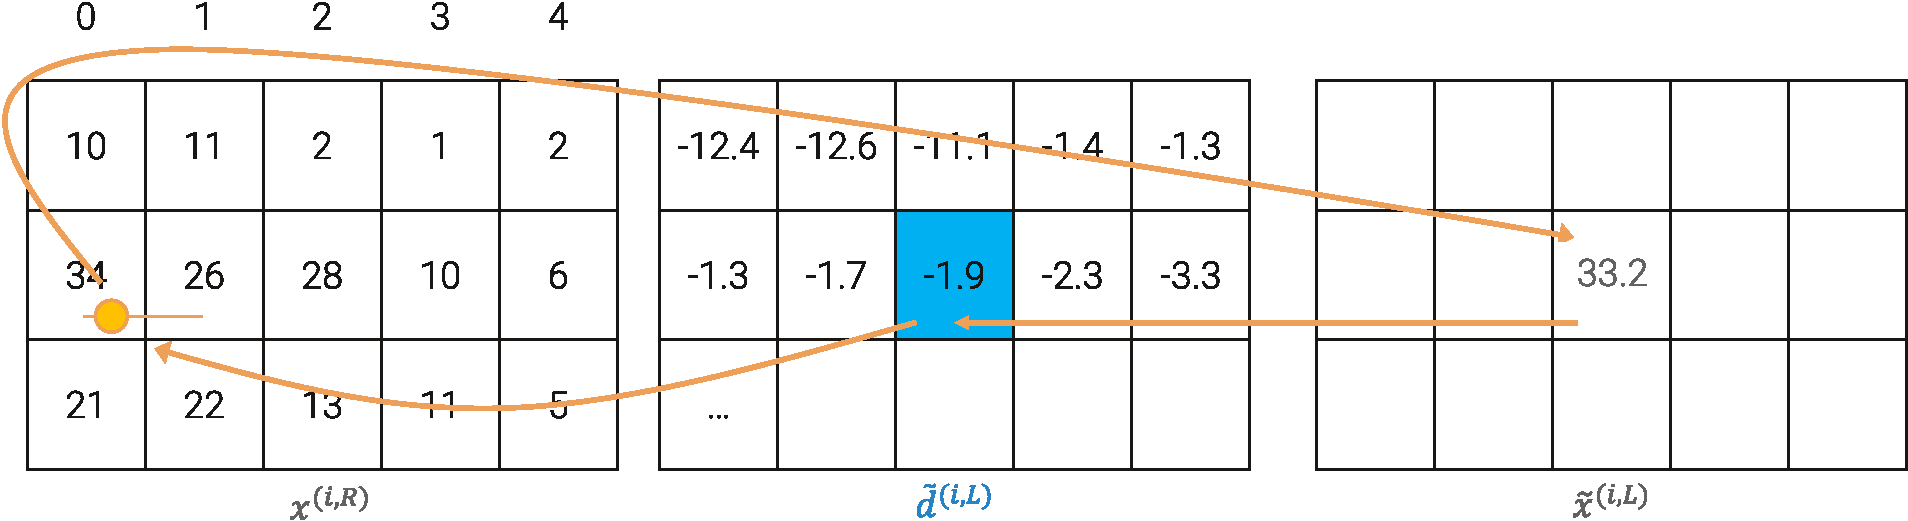
\includegraphics[width=0.65\linewidth]{./img/_monodepth_train_correct.pdf}
                    \caption{Backward reconstruction from the left image}
                \end{figure}

                \begin{figure}[H]
                    \centering
                    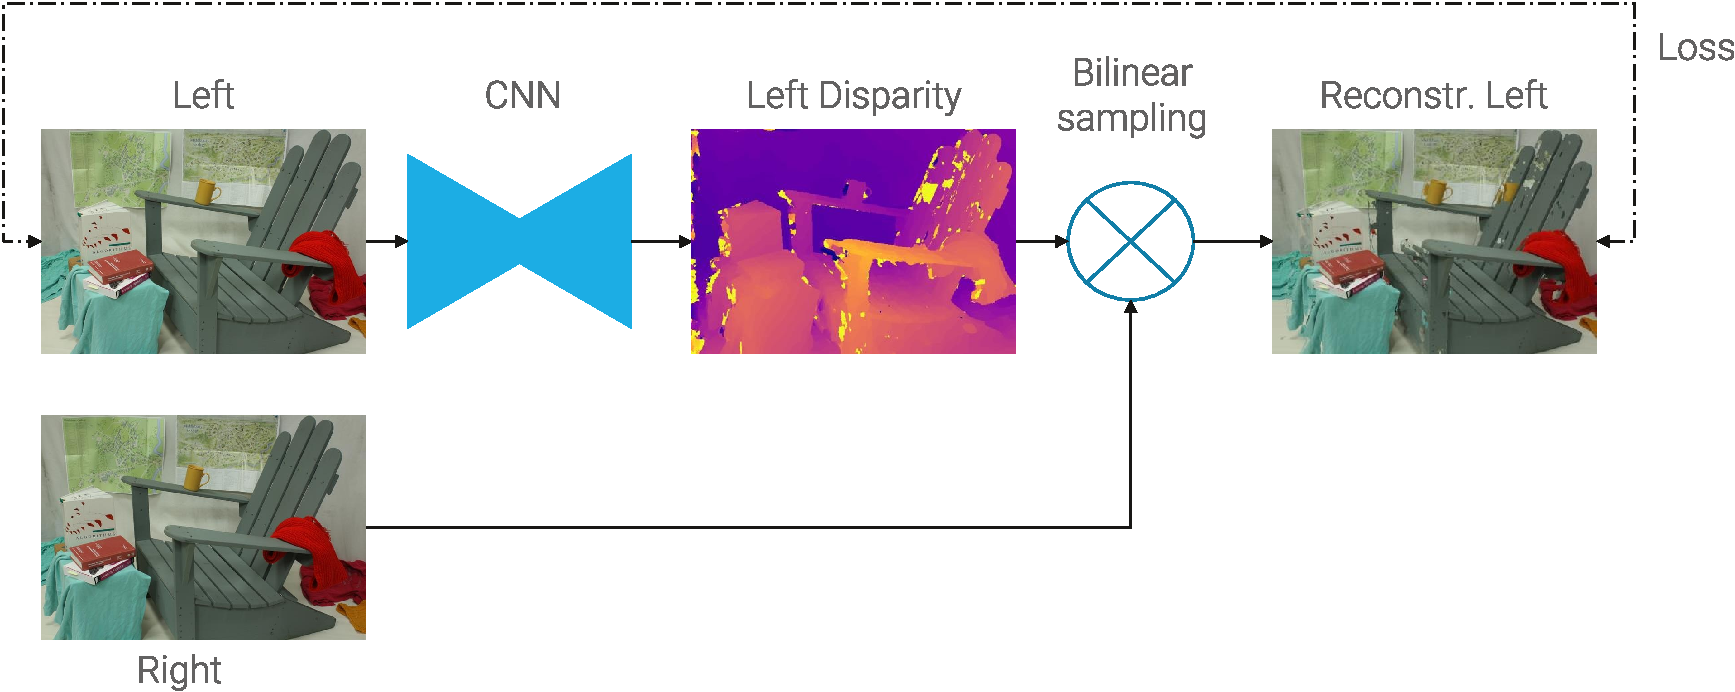
\includegraphics[width=0.7\linewidth]{./img/_monodepth_correct.pdf}
                    \caption{Actual training flow}
                \end{figure}
        \end{description}

\end{description}